% FLL block diagram
\begin{figure*}[ht]
	\centering

	% Управљачка логика
	\begin{tikzpicture}
		\clip (1.35,0.8) rectangle (10.1,4.5);
		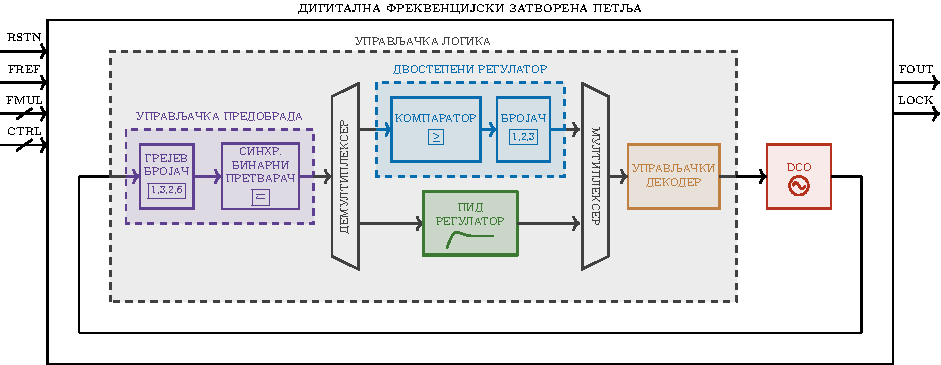
\includegraphics[scale=0.8]{slike/prezentacija/FLL.pdf}
	\end{tikzpicture}
	
	\vspace{1cm}
	% Управљачка логика: Управљачка предобрада
	\begin{tikzpicture}
		\clip (1.55,1.75) rectangle (4.4,3.55);
		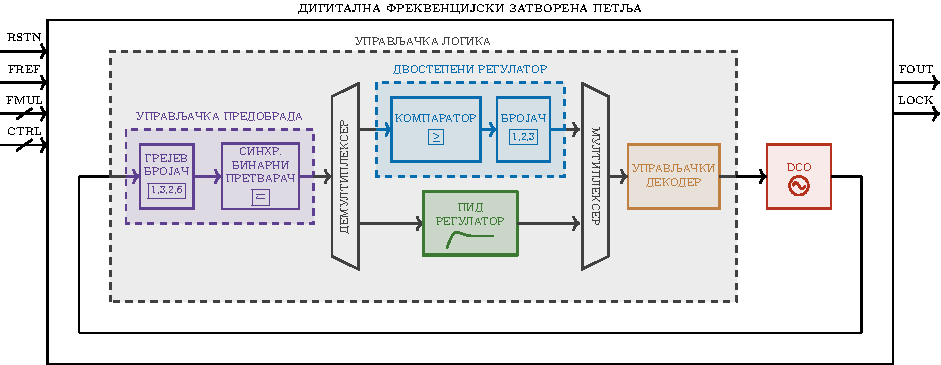
\includegraphics[scale=0.8]{slike/prezentacija/FLL.pdf}
	\end{tikzpicture}
	
	\vspace{1cm}
	% Управљачка логика: Двостепени регулатор
	\begin{tikzpicture}
		\clip (4.95,2.4) rectangle (7.75,4.2);
		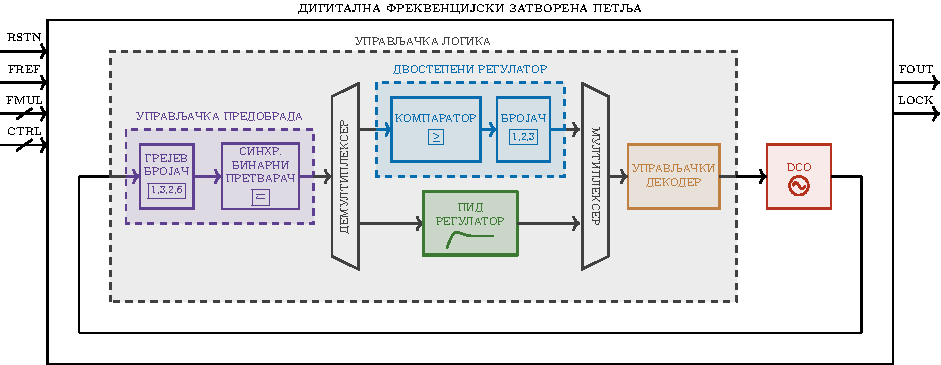
\includegraphics[scale=0.8]{slike/prezentacija/FLL.pdf}
	\end{tikzpicture}
	
	\vspace{1cm}
	% Управљачка логика: ПИД регулатор
	\begin{tikzpicture}
		\clip (5.73,1.46) rectangle (7.01,2.36);
		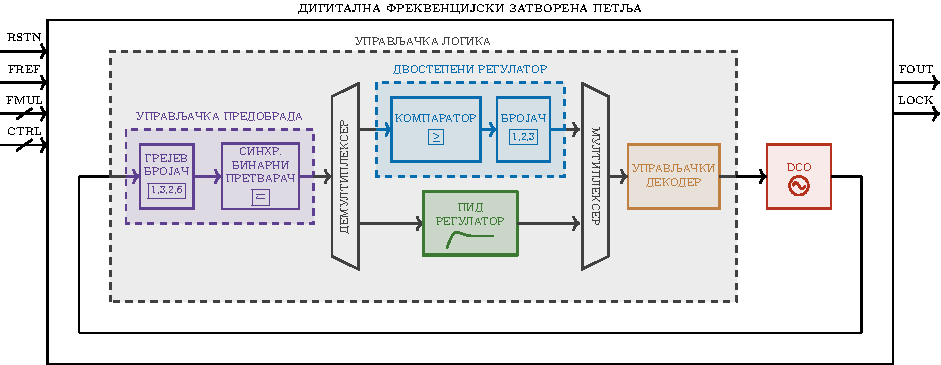
\includegraphics[scale=0.8]{slike/prezentacija/FLL.pdf}
	\end{tikzpicture}
	
	\vspace{1cm}
	% Управљачка логика: Управљачки декодер
	\begin{tikzpicture}
		\clip (8.5,2.1) rectangle (9.755,3);
		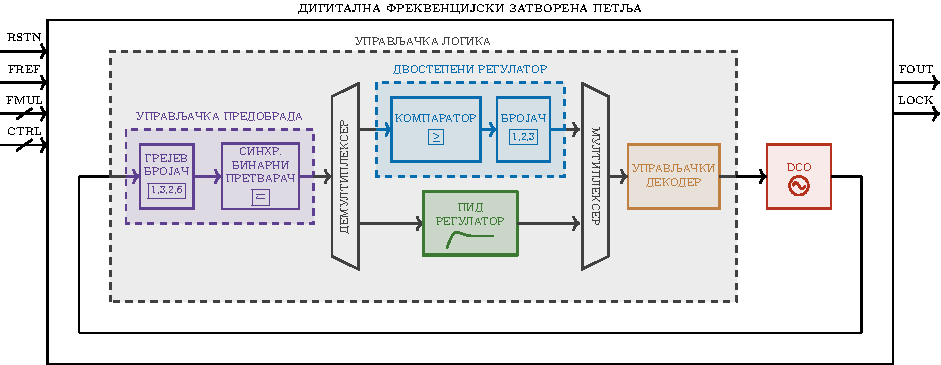
\includegraphics[scale=0.8]{slike/prezentacija/FLL.pdf}
	\end{tikzpicture}
	
	\caption{Блок дијаграм дигиталне фреквенцијски затворене петље састављене од: блока управљачке логике (лијево) и дигитално контролисаног осцилатора (десно).}
	\label{FLL block diagram}
\end{figure*}
